\subsection{适配器模式(Adapter)}

\subsubsection{适配器模式简介}

适配器模式是一种常用的设计模式。它可以将一个类的接口转换成客户希望的另外一个接口。适配器模式通过创建一个包装类,将原有类作为包装类的一个属性,来实现对原有类接口的转换。

适配器模式还可以用于解决接口不兼容的问题。例如,当我们需要使用一个第三方库中的类时,但该类的接口与我们自己的类不兼容,就可以使用适配器模式来解决这个问题。我们可以创建一个适配器类,将第三方库中的类作为适配器类的属性,并实现与我们自己的类兼容的接口。

\subsubsection{适配器模式在项目中的应用}

\begin{figure}[H]
  \centering
  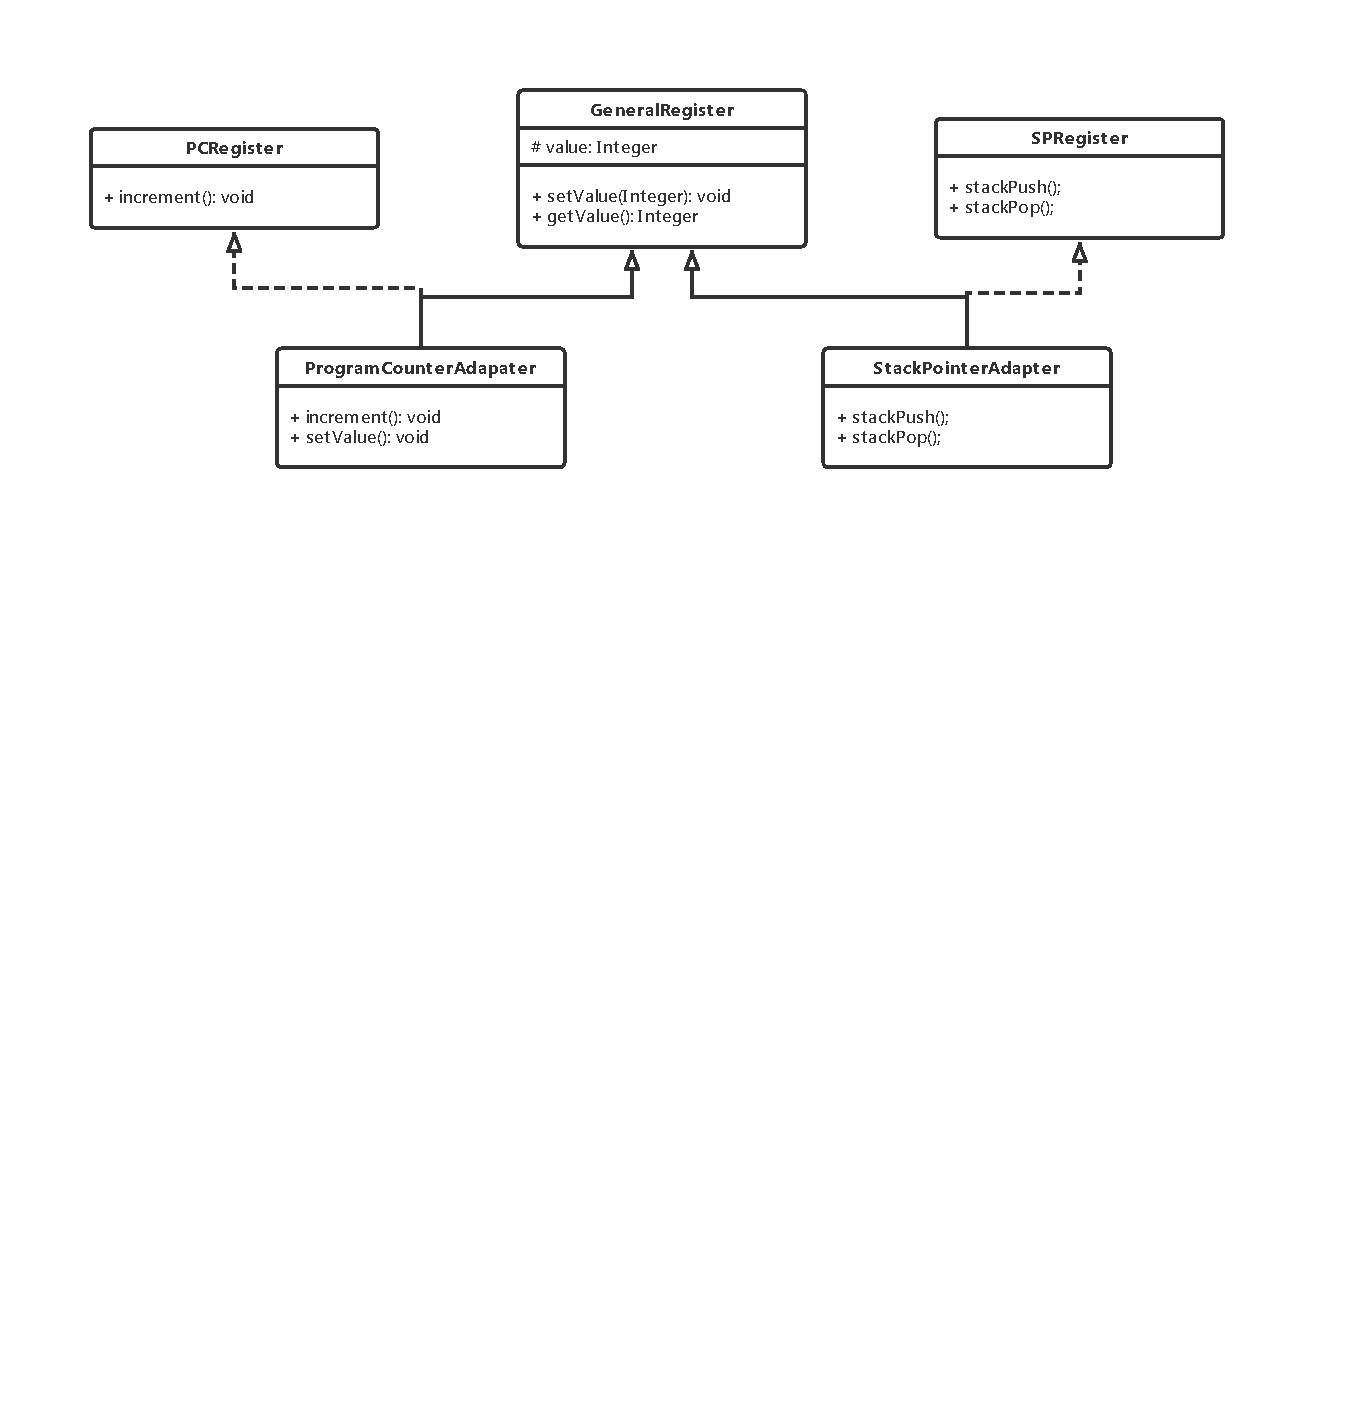
\includegraphics[width=0.9\textwidth]{figures/适配器模式.pdf}
  \caption{适配器模式在 Slow6502 中的类图}
\end{figure}

我们使用适配器模式将通用寄存器的接口改为栈寄存器和 PC 寄存器的接口。在这种情况下,可能存在一些代码依赖于通用寄存器的接口,但是你希望使用栈寄存器和 PC 寄存器。为了解决这个问题,你可以使用适配器模式来创建一个新的类,该类实现通用寄存器的接口,并将调用转发给栈寄存器和 PC 寄存器。这样,你就可以在不改变现有代码的情况下使用栈寄存器和 PC 寄存器。

总之,使用适配器模式来解决这个问题是合适的。它可以让你在不改变现有代码的情况下使用栈寄存器和 PC 寄存器,从而提高代码的灵活性和可维护性。

